% Stage 3 report, revision 4: models are described first (Sections 1-2), all results follow
% (Sections 3-5). Compile from this folder: pdflatex stage3_v4.tex (twice).
\documentclass[11pt,a4paper]{article}
\usepackage[margin=2.2cm]{geometry}
\usepackage[T1]{fontenc}
\usepackage{lmodern}
\usepackage{amsmath}
\usepackage{graphicx}
\usepackage{booktabs}
\usepackage{array}
\usepackage{enumitem}
\usepackage{xcolor}
\usepackage{caption}
\usepackage{subcaption}
\usepackage{float}
\usepackage[section]{placeins}
\usepackage[hidelinks]{hyperref}
\graphicspath{{../../experiments/}}
\setlist{itemsep=1pt,topsep=3pt}
\setlength{\parindent}{0pt}
\setlength{\parskip}{4pt}
\captionsetup{font=small,labelfont=bf}
\newcommand{\us}{\,$\mu$s}
\newcommand{\degC}{\,\textdegree C}

\begin{document}

\begin{center}
{\LARGE\bfseries Lightweight Temperature Predictor:}\\[4pt]
{\Large\bfseries TapaSense}\\[8pt]
Ethan Bobby Kurien \quad Kaivalya Mase
\end{center}

%=====================================================================
\section{Recap: the steady-state model}\label{sec:recap}
\textbf{Floorplans.} The main set is 24 floorplans: the 23 given ones and HET-A, our own
heterogeneous layout. Each has $N = 8$ cores (2 big, 6 little). Some experiments use the
\emph{main subset}, one floorplan per style: s1\_fp001, s2\_fp004, s3\_fp002 and s4\_fp001.

\textbf{S1, the influence matrix.} The steady temperature of every block is
\begin{equation}
  T = T_\text{amb} + G\,P,
  \label{eq:s1}
\end{equation}
where $P$ is the vector of core powers (W), $T_\text{amb}$ the ambient temperature, and $G$ the
\emph{influence matrix}: $G_{ij}$ is the steady temperature rise of block $i$ (K) per watt in core
$j$. Column $j$ of $G$ is measured directly by one steady run of HotSpot~\cite{hotspot}, the
reference simulator, with 1\,W in core $j$, so
8 runs (about 4\,s) calibrate a floorplan.
\begin{itemize}
  \item \textbf{Exact.} S1 reproduces HotSpot to its 6-decimal output (0.00003\,K worst on 7{,}248
        test runs) and always picks the right hottest core.
  \item \textbf{Cheap.} One matrix--vector product per prediction (2.6\us) and 928\,B per
        floorplan (464\,B in 32-bit numbers).
  \item \textbf{Calibration is needed.} Every calibration-free alternative (a generic heat-spread
        kernel, or $G$ borrowed from another floorplan or predicted from geometry) was 0.5--2.7\,K
        off on average and up to 12\,K.
\end{itemize}

%=====================================================================
\section{Transient models}\label{sec:models}
This section describes the transient models and how each is calibrated.

\subsection{Calibration data: planned step runs}\label{sec:steps}
Because HotSpot is linear, its temperature response to any power trace is \emph{fixed by the
response to a 1\,W step in each core}. Transient calibration therefore records these step responses.

\subsection{T1: one time constant (baseline)}
The simplest transient model lets each block move a fixed fraction of the way towards its S1
steady value at every time step:
\begin{equation}
  x_i[k+1] = a_i\, x_i[k] + (1 - a_i)\,(G\,P[k])_i, \qquad a_i = e^{-\Delta t/\tau_i},
  \qquad T_i = T_\text{amb} + x_i,
  \label{eq:t1}
\end{equation}
where $x_i$ is block $i$'s rise above ambient, $\Delta t$ the time step at which the model predicts
(1\,ms), and $\tau_i$ one time constant per block, fitted so that its step response
$G_{ij}(1 - e^{-t/\tau_i})$ is as close as possible to the measured step responses $s_{ij}(t)$
(Section~\ref{sec:t3}).

\subsection{T3: sum of exponentials}\label{sec:t3}
Each step response is written as a sum of $M$ rising curves:
\begin{equation}
  s_{ij}(t) \approx \sum_{m=1}^{M} a_{ijm}\left(1 - e^{-t/\tau_m}\right),
  \qquad \sum_m a_{ijm} = G_{ij}.
  \label{eq:t3}
\end{equation}
\textbf{What $s_{ij}(t)$ is.} $s_{ij}(t)$ is the temperature rise of core $i$ at time $t$ after
1\,W is switched on in core $j$. It is the transient version of the influence-matrix entry: it
starts at 0 and, once the chip settles, ends at $G_{ij}$, so $s_{ij}(\infty) = G_{ij}$. The
responses mix very different speeds, from about a millisecond (the silicon under a core) to many
seconds (the heat sink); a \emph{time constant} $\tau$ is how long one of these parts takes to cover
about two-thirds of its rise.
\begin{itemize}
  \item \textbf{The curves $1 - e^{-t/\tau_m}$ are the same for every pair of cores.} The $M$ time
        constants $\tau_1, \dots, \tau_M$ belong to the chip and package (silicon, spreader, sink),
        not to a particular pair.
  \item \textbf{Only the weights $a_{ijm}$ differ between pairs.} They say how much of the
        $i \leftarrow j$ heating happens at each speed.
  \item \textbf{The weights of each pair add up to $G_{ij}$}, so T3 ends at exactly S1's value:
        it is exact in steady state.
\end{itemize}

\subsection{T2: ARX, calibrated from one long trace}\label{sec:arx}
Instead of planned steps, ARX is fitted to one long
recorded HotSpot trace. It is a standard way to build a model of a system from its recorded inputs
(here the powers) and outputs (the temperatures) alone, and it has also been used for temperature
prediction in~\cite{coskun09,singla15}.

\textbf{Calibration trace.} 60\,s at 1\,ms steps on each main-subset floorplan, from a cold chip.
Every core switches independently between random power levels, with phases of 1\,ms to 5\,s, so
both fast and slow behaviour is excited.

\textbf{The model.} The next temperature rise above ambient is a weighted mix of the last few rises
and powers. With $n_a$ past rises and $n_b$ powers, written ARX$(n_a, n_b)$:
\begin{equation}
  x[k] = \sum_{l=1}^{n_a} A_l\, x[k-l] + \sum_{l=0}^{n_b-1} B_l\, P[k-l].
  \label{eq:arx}
\end{equation}
For example, ARX(2,2) is
\[
  x[k] = A_1 x[k-1] + A_2 x[k-2] + B_0 P[k] + B_1 P[k-1].
\]
Here $x$ is the vector of rises, of every block (``all blocks'') or of the 8 cores only (``cores
only'', which is what on-chip sensors measure); $A_l$ and $B_l$ are matrices of coefficients.

\textbf{Exact in steady state, but not always stable.} The coefficients are constrained so that,
for constant power, ARX settles at exactly S1's $G\,P$. This fixes \emph{where} ARX settles, not
\emph{whether} it settles.

%=====================================================================
\section{Results}\label{sec:results}

\subsection{Fit to the step responses (calibration data)}
This is how closely each model reproduces the step runs it was calibrated on; the error is the
largest difference from HotSpot over the response to switching on the nominal power of all cores
(the power level given with the dataset: 20\,W per big core and 8\,W per little core, 88\,W in
total). Errors on unseen test traces follow in Section~\ref{sec:follow}.

The step responses span very different speeds: the six time constants fitted with $M = 6$ are about
1\,ms, 3\,ms, 26\,ms, 89\,ms, 0.56\,s and 8.1\,s.

\begin{center}
\small
\begin{tabular}{@{}l c c@{}}
\toprule
Model & Worst fit error, main set (24 floorplans) & Size \\
\midrule
T1 (one time constant per block) & 14.1\,K & 1.0\,kB \\
T3, $M=2$ & 2.82\,K & 1.9\,kB \\
T3, $M=3$ & 1.04\,K & 2.8\,kB \\
T3, $M=4$ & 0.46\,K & 3.7\,kB \\
T3, $M=6$ & 0.12\,K & 5.6\,kB \\
\bottomrule
\end{tabular}
\end{center}
One time constant (T1) cannot follow a response spanning 1\,ms to 8\,s. T3 converges quickly with
$M$.

\begin{figure}[H]
  \centering
  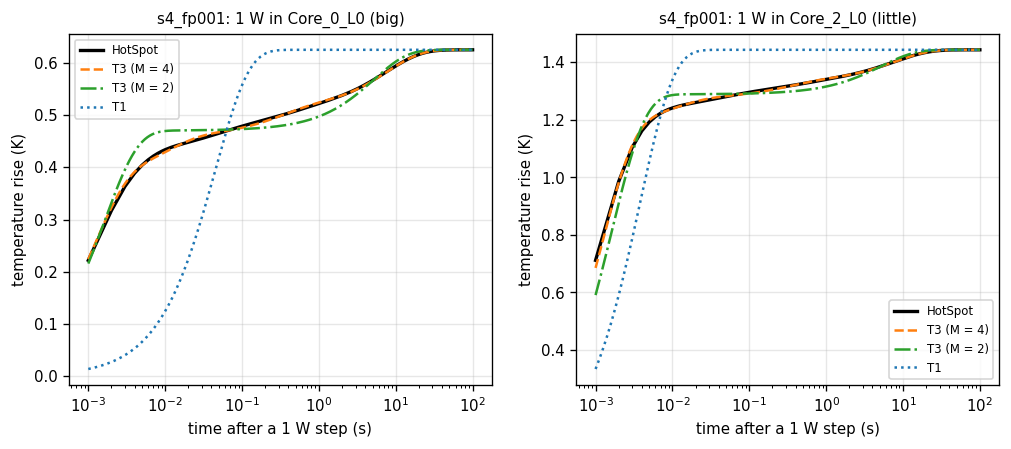
\includegraphics[width=0.9\linewidth]{P1-1_step_calibration/results/step_response_fits_stage3.png}
  \caption{Step responses to 1\,W in a big core (left) and a little core (right), log time axis.}
  \label{fig:steps}
\end{figure}

\subsection{Following HotSpot over time}\label{sec:follow}
Tested from a cold chip on a 2\,s trace on each of the 24 floorplans, plus two longer 10\,s traces
on each of the four main-subset floorplans, and on a real workload (HotSpot's EV6 floorplan with a
gcc power trace).

\begin{center}
\small
\begin{tabular}{@{}l c c c c@{}}
\toprule
Model & Mean error & Worst error & Time per step & Size \\
\midrule
T1 & 7.25\,K & 14.6\,K & 1.5\us & 1.0\,kB \\
T3, $M=2$ & 0.92\,K & 2.9\,K & 3.0\us & 1.9\,kB \\
T3, $M=3$ & 0.19\,K & 1.1\,K & 3.0\us & 2.8\,kB \\
T3, $M=4$ & 0.090\,K & 0.30\,K & 3.1\us & 3.7\,kB \\
T3, $M=6$ & 0.0093\,K & 0.13\,K & 3.2\us & 5.6\,kB \\
T2 ARX (main subset) & 0.19\,K & 0.57\,K & 5.4\us & 6.2\,kB \\
T3 $M=4$ on EV6 + gcc & 0.073\,K & 0.21\,K & 4.4\us & 28.8\,kB \\
\bottomrule
\end{tabular}
\end{center}
Increasing $M$ improves accuracy at the cost of model size; no speed-up or slow-down is observed.

\begin{figure}[H]
  \centering
  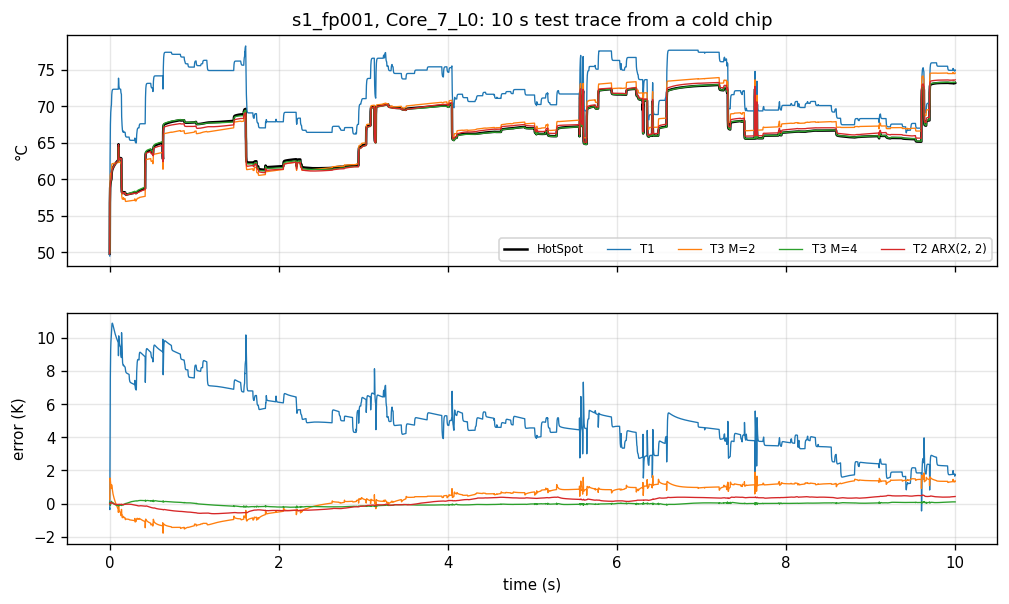
\includegraphics[width=0.75\linewidth]{P3-1_transient_predictor/results/trace_example.png}
  \caption{HotSpot and the models on one 10\,s test trace from a cold chip (top) and their error (bottom); T3 sits on top of HotSpot.}
  \label{fig:trace}
\end{figure}

\subsection{Trade-offs}
Figure~\ref{fig:pareto} collects every model's size, worst error and speed. In the transient case
(a), T3 alone forms the Pareto front from $M = 4$ on (0.31\,K worst error and below). At 2--3\,kB, cores-only ARX
is on the front next to T3 with $M = 2$--3, but all of these are about 1--3\,K off at worst. In
steady state (b) there is no trade-off: S1 is exact already at 464\,B (32-bit numbers), and every
smaller model (the compressed S2 variants of Stage 2) is kelvins off.

\begin{figure}[H]
  \centering
  \begin{subfigure}{0.495\linewidth}
    \centering
    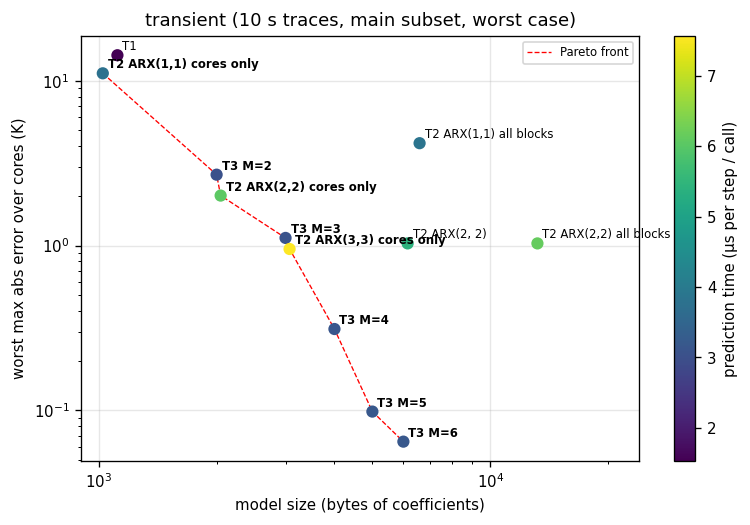
\includegraphics[width=\linewidth]{P3-3_pareto/results/pareto_transient.png}
    \caption{Transient models.}
  \end{subfigure}\hfill
  \begin{subfigure}{0.495\linewidth}
    \centering
    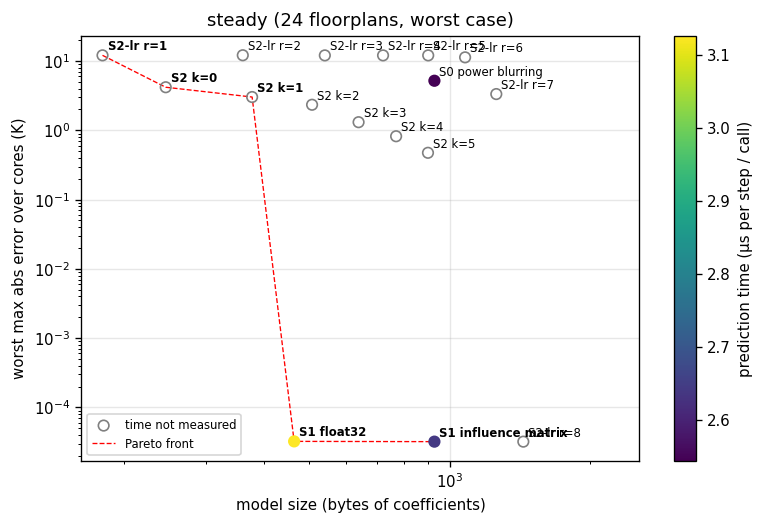
\includegraphics[width=\linewidth]{P3-3_pareto/results/pareto_steady.png}
    \caption{Steady models.}
  \end{subfigure}
  \caption{Model size against worst error; colour is the prediction time per step (transient) or
  per call (steady). Bold labels and the red dashed line: the Pareto front (no other model is both
  smaller and more accurate).}
  \label{fig:pareto}
\end{figure}

%=====================================================================
\section{The final transient model}

\subsection{T3 with four time constants}
The transient model is T3 with $M=4$ (Equation~\eqref{eq:t3}). Of the three families (T1, ARX
and T3), we chose it because:
\begin{itemize}
  \item it meets the targets with room to spare: 0.09\,K mean and 0.30\,K worst error against
        0.5\,K and 1\,K, at 3.1\us\ per step and 3.7\,kB;
  \item it is exact in steady state and cannot become unstable, unlike ARX;
  \item it gives the best accuracy per byte, and $M$ is one knob for more accuracy ($M=6$: 0.13\,K
        worst for 5.6\,kB).
\end{itemize}
T1 was ruled out because one time constant cannot cover 1\,ms to 8\,s (14\,K worst), and ARX
because it is about 2$\times$ less accurate (0.19\,K mean and 0.57\,K worst error), needs a long
recorded trace, and can be unstable.

\subsection{Testing on 52 generated floorplans}\label{sec:gen}
The models were developed and evaluated on the 24 floorplans of the main set. To check that these
were not a lucky set, we tested them on floorplans they had never seen:
\begin{itemize}
  \item \textbf{Floorplans.} Our generator produced 13 floorplans in each of the four given styles
        (52 in total), with the same cores (2 big, 6 little), the same file format and layer
        stack, and placement rules that imitate each style.
  \item \textbf{Tests.} T3 on a 2\,s phase trace from a cold chip, in which every core switches
        between power levels in phases of 1\,ms to 2\,s.
\end{itemize}

\begin{center}
\small
\begin{tabular}{@{}l c c c@{}}
\toprule
Style & Floorplans & T3 mean & T3 worst \\
\midrule
Style 1 & 13 & 0.108\,K & 0.34\,K \\
Style 2 & 13 & 0.114\,K & 0.32\,K \\
Style 3 & 13 & 0.085\,K & 0.31\,K \\
Style 4 & 13 & 0.056\,K & 0.26\,K \\
All generated & 52 & 0.091\,K & 0.34\,K \\
Main set (24 floorplans) & 24 & 0.090\,K & 0.30\,K \\
\bottomrule
\end{tabular}
\end{center}

\begin{figure}[H]
  \centering
  \begin{subfigure}{\linewidth}
    \centering
    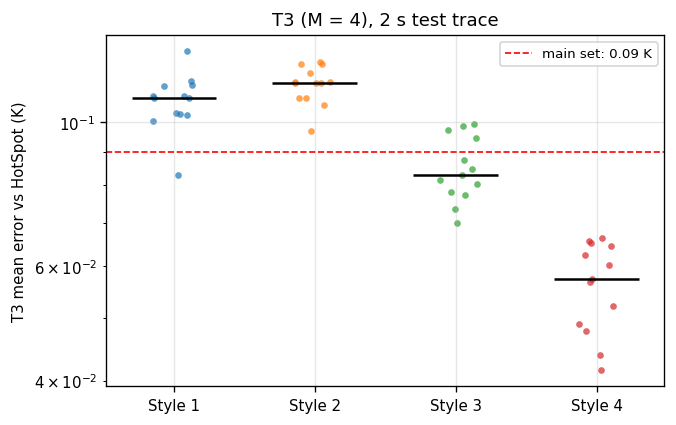
\includegraphics[width=0.6\linewidth]{extended_validation/results/error_by_style_t3.png}
    \caption{T3's mean error per generated floorplan (one dot each); black bar = median of the
    style, red line = main set.}
  \end{subfigure}
  \caption{Validation on the 52 generated floorplans.}
\end{figure}

\begin{figure}[H]
  \ContinuedFloat
  \centering
  \begin{subfigure}{\linewidth}
    \centering
    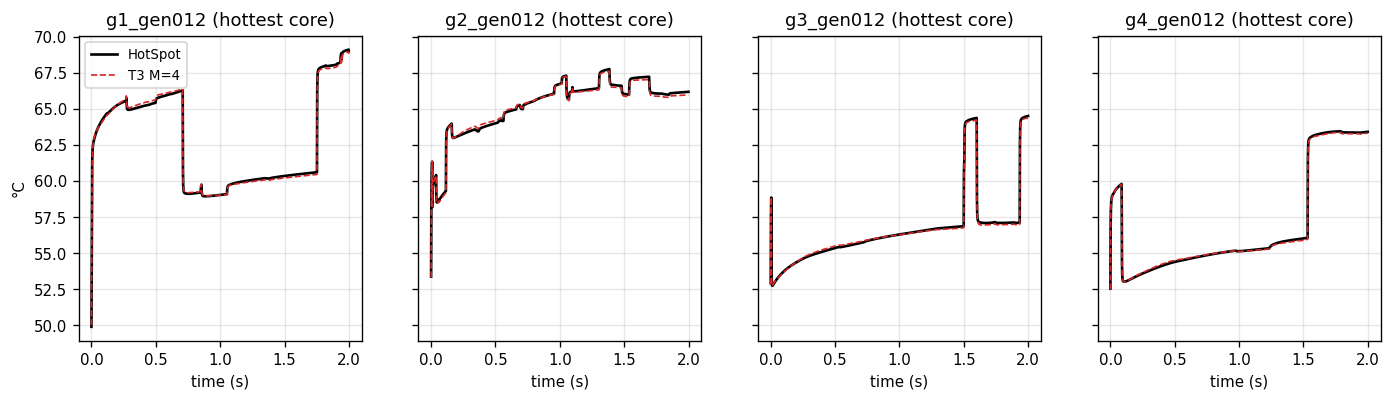
\includegraphics[width=\linewidth]{extended_validation/results/transient_check.png}
    \caption{The hottest core of one generated floorplan per style on its 2\,s test trace; T3
    (red dashed) follows HotSpot (black).}
  \end{subfigure}
  \caption[]{Validation on the 52 generated floorplans (continued).}
\end{figure}

\begin{figure}[H]
  \centering
  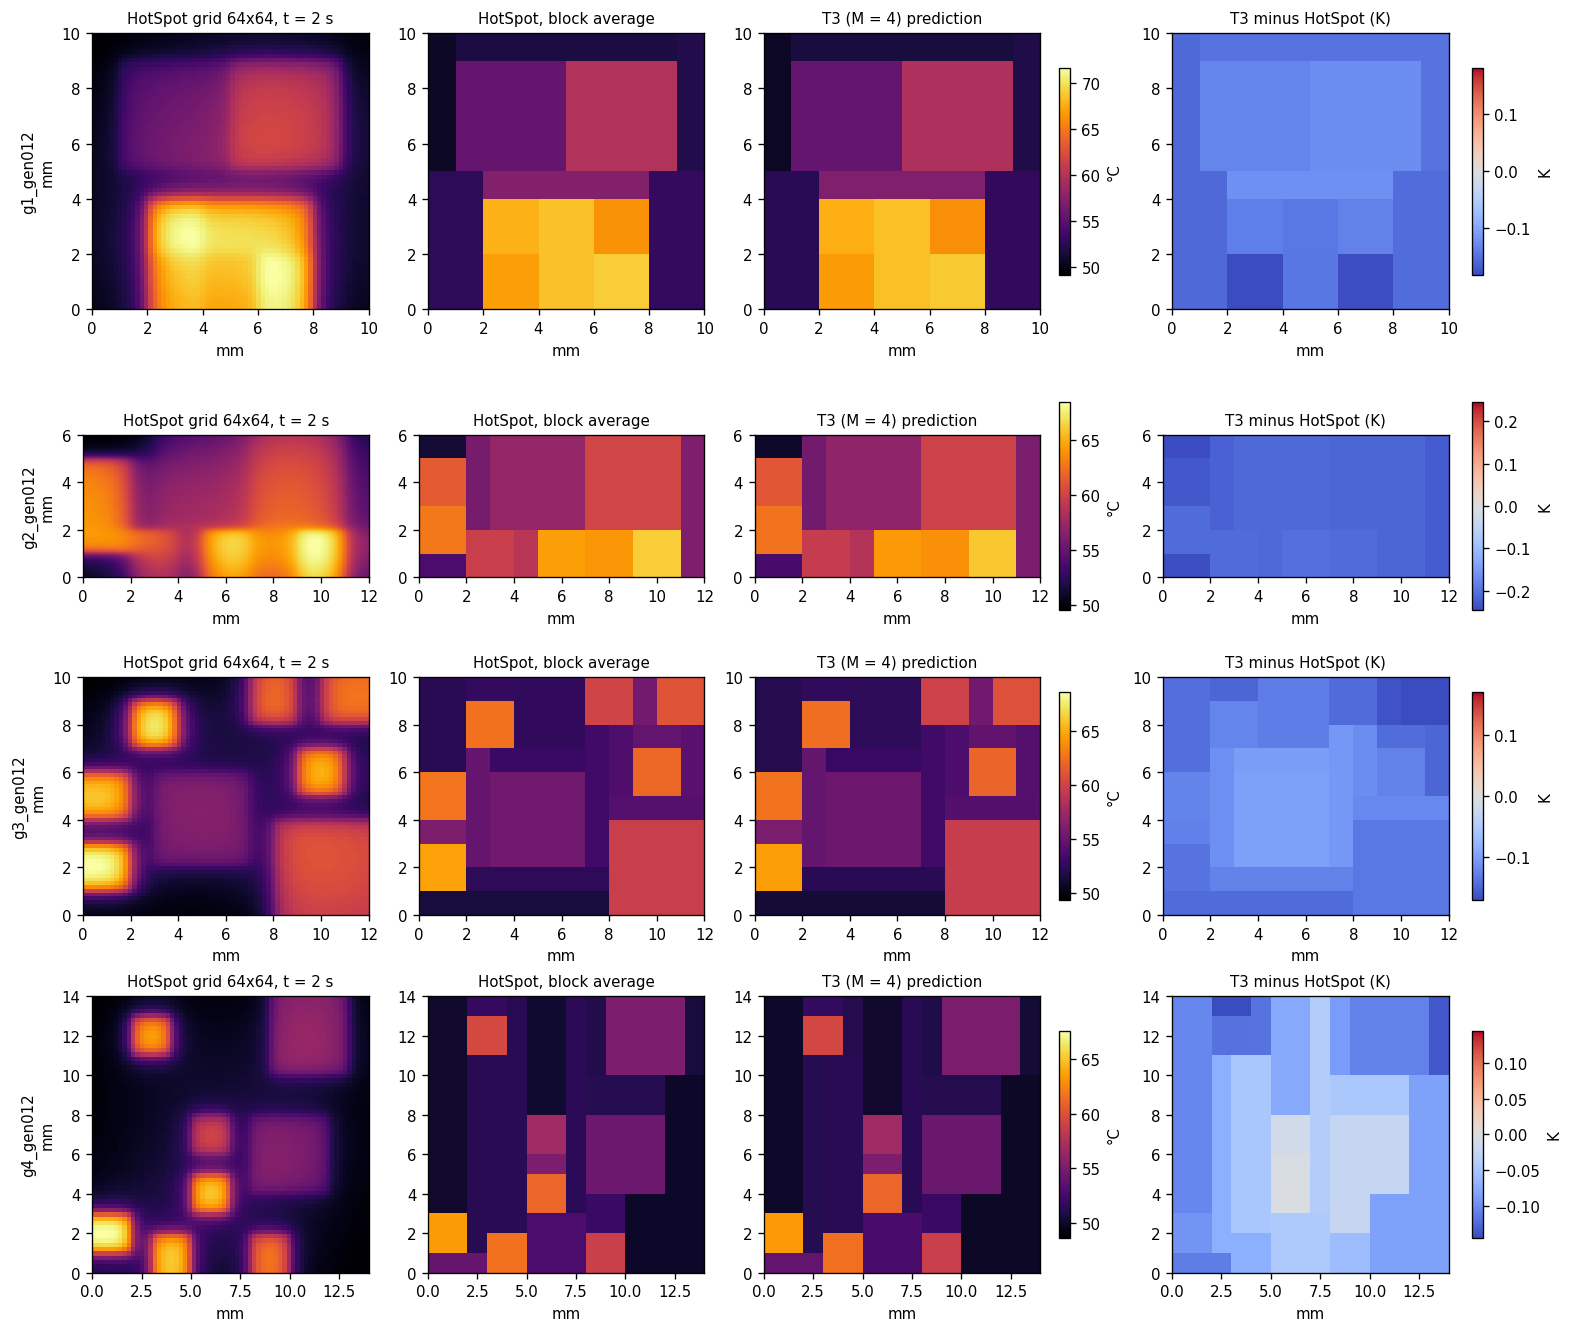
\includegraphics[width=\linewidth]{extended_validation/results/heatmaps_t3.png}
  \caption{T3 at the end of the 2\,s test trace, one generated floorplan per style. Columns:
  HotSpot's $64\times64$ map; HotSpot's block averages; T3's prediction (same colour scale); T3
  minus HotSpot in kelvin.}
  \label{fig:maps}
\end{figure}

\textbf{The results carry over.} Over 52 new floorplans T3 is off by 0.09\,K on average, the same as
on the main set.

%=====================================================================
\section{Robustness}

\subsection{Unusual inputs}
\begin{center}
\small
\begin{tabular}{@{}l c c l@{}}
\toprule
Case (main subset) & T3 mean & T3 worst & Verdict \\
\midrule
Normal trace (reference) & 0.10\,K & 0.32\,K & fine \\
Steady power at 3$\times$ the maximum (S1) & 0.00002\,K & 0.00005\,K & fine \\
Transient at 2$\times$ power & 0.21\,K & 0.64\,K & fine \\
Bursty power, switching every 1--5\,ms & 0.11\,K & 0.44\,K & fine \\
Task migration between cores$^{a}$ & 0.076\,K & 0.31\,K & fine \\
Warm start (after the first 50\,ms)$^{b}$ & 0.029\,K & 0.27\,K & fine \\
\bottomrule
\end{tabular}

\smallskip
\begin{minipage}{0.9\linewidth}\footnotesize
$^{a}$ One heavy task (top of its power range) moves to another core every 300\,ms, alternating
between big and little cores, while the other cores idle at the bottom of their range (3\,s).\\
$^{b}$ HotSpot and T3 both start from the steady state of the first power value instead of a cold
chip. The worst error is counted after the first 50 steps (50\,ms); over the very first steps it is
2.0\,K.
\end{minipage}
\end{center}
The coefficients are properties of the chip, and hence power levels, bursty power and workload
mapping do not change the relative error.

\subsection{Prediction for package changes}
The coefficients belong to one floorplan \emph{and} one package. Setup:
\begin{itemize}
  \item \textbf{Floorplans:} s1\_fp001 and s4\_fp001.
  \item \textbf{Three package changes}, one at a time:
  \begin{itemize}
    \item ambient 35\degC\ instead of 45\degC;
    \item heat-sink convection resistance doubled (0.1 to 0.2\,K/W, a worse cooler);
    \item heat-sink convection resistance halved (0.05\,K/W, a better cooler).
  \end{itemize}
  \item \textbf{Models:} the old models (S1 and T3, $M=4$) and models recalibrated with the usual
        24 runs under the new package.
  \item \textbf{Tests:} 50 random steady power vectors and a 3\,s trace from a cold chip.
\end{itemize}

\begin{center}
\small
\begin{tabular}{@{}l l c c@{}}
\toprule
Change & Model & Steady worst & Transient worst (3\,s) \\
\midrule
Ambient 35\degC & old model, old $T_\text{amb}$ & 10.0\,K & 10.2\,K \\
 & old model, new $T_\text{amb}$ & 0.00001--0.00002\,K & 0.23--0.27\,K \\
 & recalibrated & 0.00001--0.00002\,K & 0.23--0.27\,K \\
\midrule
Convection resistance $\times 2$ & old model & 8.5\,K & 0.43--0.48\,K \\
 & recalibrated & 0.00001--0.00002\,K & 0.26--0.29\,K \\
\midrule
Convection resistance $\times 0.5$ & old model & 4.4\,K & 0.42--0.48\,K \\
 & recalibrated & 0.00002\,K & 0.20--0.22\,K \\
\bottomrule
\end{tabular}
\end{center}
\begin{itemize}
  \item \textbf{A new ambient needs no recalibration.} The models predict the rise above ambient.
        Forgetting to update $T_\text{amb}$ results in a 10\,K error.
  \item \textbf{A new heat sink needs recalibration.} The old coefficients are 8.5\,K off in steady
        state when the convection resistance doubles and 4.4\,K when it halves; 24 runs under the
        new package restore the accuracy.
\end{itemize}

\subsection{Leakage}
Real chips leak more power when hot, which breaks linearity. Leakage current grows roughly
exponentially with temperature~\cite{liao05}, and HotSpot's leakage model~\cite{hotspot6} (steady
state only) makes every block of the silicon layer, white space included, leak
\begin{equation}
  P_{\text{leak},i}(T_i) = \alpha\, A_i\, e^{\beta\,(T_i - 383.15\,\text{K})},
  \qquad \alpha = 1.5\times10^{4}\,\text{W/m}^2,\ \beta = 0.036\,\text{K}^{-1},
  \label{eq:leak}
\end{equation}
where $A_i$ is the block's area; $\alpha$ and $\beta$ are HotSpot's default values, so leakage
doubles about every 19\,K. HotSpot iterates power and temperature until they settle. At our
temperatures this is small (0.2--0.5\,W per chip), so we also built a HotSpot with 10$\times$
$\alpha$ (2--5\,W, 3--5\,\% of chip power). Test: main subset, 50 random power vectors each, in
both builds.

\textbf{The fix to S1.} The chip is still linear in the \emph{total} power, so the calibrated
coefficients stay valid; only the leakage has to be added as extra power. Since the white-space
blocks leak too, $G$ is extended to $G_\text{all}$, with one column for every block of the silicon
layer. Starting from the plain S1
prediction $T^{(0)} = T_\text{amb} + G\,P$, the loop repeats
\begin{equation}
  T^{(k+1)} = T_\text{amb} + G_\text{all}\left(P + P_\text{leak}\big(T^{(k)}\big)\right)
  \label{eq:leakloop}
\end{equation}
until the temperatures change by less than $10^{-4}$\,K.

\begin{center}
\small
\begin{tabular}{@{}l c c c c c@{}}
\toprule
Leakage & Leakage power & S1 alone (worst) & S1 + loop (worst) & Iterations & Time \\
\midrule
Default & 0.2--0.5\,W & 0.08--0.10\,K & $1$--$2\times10^{-5}$\,K & 3 & 22--25\us \\
10$\times$ stronger & 2--5\,W & 0.77--1.07\,K & $2$--$6\times10^{-5}$\,K & 4 & 29--33\us \\
\bottomrule
\end{tabular}
\end{center}
Ignoring leakage costs about 0.1\,K at default strength and 1\,K at 10$\times$. The loop removes
the error completely, back to HotSpot's output precision, in 3--4 iterations; it is about
10$\times$ slower than S1 alone but still about 10{,}000$\times$ faster than one HotSpot run.
HotSpot does not support leakage in transient runs, so the transient side could not be tested.

%=====================================================================
\section{The tool: \texttt{ltp}}
Both stages are available as commands that need only NumPy and a model file:
{\small\begin{verbatim}
# Run the 24 HotSpot calibration runs for floorplan s4_fp001, fit S1, T3 and the
# hot-spot rows, and save them in one model file.
python3 -m src.ltp calibrate s4_fp001 -o model_s4_fp001.npz

# Steady temperatures (deg C) of every block for these 8 core powers (W).
python3 -m src.ltp steady    model_s4_fp001.npz --power 20,20,8,8,8,8,8,8

# Run T3 on a HotSpot power trace and write the predicted temperature trace.
python3 -m src.ltp transient model_s4_fp001.npz --ptrace trace.ptrace -o out.ttrace

# Check the model against fresh HotSpot runs: accuracy, speed and size.
python3 -m src.ltp bench     model_s4_fp001.npz s4_fp001
\end{verbatim}}
The given \texttt{.ptrace} files are read directly, and transient output is a HotSpot-style
\texttt{.ttrace}.

\textbf{Example check with \texttt{bench}.} On s4\_fp001, \texttt{bench} runs HotSpot on 300 new
steady power vectors and a 2\,s test trace and compares the model with it:
\begin{itemize}
  \item the model file holds 8{,}032\,B of coefficients ($G$, T3 and the hot-spot rows);
  \item steady state: $5.2\times10^{-6}$\,K mean and $1.4\times10^{-5}$\,K worst error, 2.6\us\
        per prediction;
  \item transient: 0.051\,K mean and 0.189\,K worst error, 3.5\us\ per time step.
\end{itemize}

%=====================================================================
\section{What went as planned, and what deviated}
\textbf{As planned:} the two-stage design; HotSpot grid model as the reference; S1 as the steady
model with 8 runs; T3 as the transient model; evaluation on accuracy, time and size; the
calibration-is-needed check; robustness studies; the \texttt{ltp} tool. All steady and transient
targets were met, except calibration wall time (about 2.75\,min per floorplan against a target of
2\,min).

\begin{center}
\small
\begin{tabular}{@{}p{3cm} p{4.3cm} p{7.7cm}@{}}
\toprule
Item & Planned & Done, and why \\
\midrule
HotSpot build & Precision patch & Also LU caching (29$\times$ faster) and a memory-leak fix: a 60\,s trace took 4\,h or ran out of memory. \\
Dataset & Our synthetic floorplans & The 23 given floorplans (plus HET-A) as the main set, plus 52 generated in the same styles. \\
Hot spots & One hottest cell per core & S1-hot-max over all cells of a core, which is exact, compressed by dropping cells that can never be the hottest. \\
\bottomrule
\end{tabular}
\end{center}

%=====================================================================
\section{Pending items (for Stage 4)}
\begin{itemize}
  \item Package \texttt{ltp} for \texttt{pip install}.
  \item Final report, code archive, README with run instructions, and presentation feedback.
\end{itemize}

%=====================================================================
\section{Learnings from Stage 3}
\begin{enumerate}
  \item Heat moves on time scales from 1\,ms to 8\,s; one time constant cannot capture this.
  \item Planned step runs beat fitting a recorded trace, by about 2$\times$ and with guaranteed
        stability.
  \item Changing the package (the heat sink) requires recalibration; a new ambient temperature
        does not.
  \item Engineering the reference was a prerequisite for every experiment. HotSpot as shipped
        prints temperatures to 0.01\,K, while we needed to measure errors of $10^{-5}$\,K, so we
        patched it to print 6 decimals; caching its matrix factorisation made it 29$\times$
        faster; and a memory-leak fix was needed because a 60\,s trace took 4\,h or ran out of
        memory.
\end{enumerate}

%=====================================================================
\section{Future scope}
\begin{itemize}
  \item Leakage in transient prediction, with a simulator that supports it.
  \item Hot-spot models that scale to many cores.
  \item Calibration from real sensor measurements instead of a simulator; T3 and S1 only need
        input--output data, so the method carries over.
\end{itemize}

%=====================================================================
\section{LLM assistance disclosure}
LLMs were used to understand HotSpot, for literature review to select appropriate models, generate
floorplans, and calibration and testing scripts.

\begin{thebibliography}{99}\small
\setlength{\itemsep}{0pt}
\bibitem{hotspot} W.~Huang, S.~Ghosh, S.~Velusamy, K.~Sankaranarayanan, K.~Skadron and
  M.~R. Stan, ``HotSpot: A Compact Thermal Modeling Methodology for Early-Stage VLSI Design,''
  \emph{IEEE TVLSI} 14(5):501--513, 2006.
\bibitem{hotspot6} R.~Zhang, M.~R. Stan and K.~Skadron, ``HotSpot 6.0: Validation, Acceleration
  and Extension,'' Univ. of Virginia, Tech. Rep. CS-2015-04, 2015.
\bibitem{liao05} W.~Liao, L.~He and K.~M. Lepak, ``Temperature and Supply Voltage Aware
  Performance and Power Modeling at Microarchitecture Level,'' \emph{IEEE TCAD} 24(7):1042--1053,
  2005.
\bibitem{coskun09} A.~K. Coskun, T.~S. Rosing and K.~C. Gross, ``Utilizing Predictors for
  Efficient Thermal Management in Multiprocessor SoCs,'' \emph{IEEE TCAD} 28(10), 2009.
\bibitem{singla15} G.~Singla, G.~Kaur, A.~K. Unver and U.~Y. Ogras, ``Predictive Dynamic Thermal
  and Power Management for Heterogeneous Mobile Platforms,'' in \emph{Proc. DATE}, 2015.
\end{thebibliography}

\end{document}
